% BER+ Coordination Map — June 12 leadership briefing (camera-ready)
% Compile: pdflatex june12-final.tex  (twice if needed)
% Live demo: https://ber-war-map.vercel.app/

\documentclass[aspectratio=169,11pt]{beamer}
\usetheme{Madrid}
\usecolortheme{seahorse}
\usepackage[utf8]{inputenc}
\usepackage[T1]{fontenc}
\usepackage{graphicx}
\usepackage{booktabs}
\usepackage{hyperref}

\hypersetup{colorlinks=true, linkcolor=blue, urlcolor=teal}
\newcommand{\demourl}{\url{https://ber-war-map.vercel.app/}}
\newcommand{\berhub}{BER+ Board Room}

\title{BER+ Board Room}
\subtitle{Matching · visibility · corridor intelligence — ecosystem coordination, not command centres}
\author{BER+ Flughafenregion}
\institute{Schönefeld corridor · Flughafenregion Berlin Brandenburg}
\date{12 June 2026}

\graphicspath{{figures/}}

\begin{document}

% --- Title ---
\begin{frame}
  \titlepage
  \vfill
  \centering\demourl
\end{frame}

% --- Agenda ---
\begin{frame}{Agenda}
  \begin{enumerate}
    \item \textbf{The problem} --- fragmented visibility in the Flughafenregion
    \item \textbf{Why now} --- strategic choice \& benchmarks
    \item \textbf{Live demo} --- company · investor · municipality on the map
    \item \textbf{What BER+ does} --- pilot phase, asset inventory, next steps
  \end{enumerate}
  \vfill
  \small\demourl
\end{frame}

% --- Problem ---
\begin{frame}{The problem --- information is fragmented}
  \begin{itemize}
    \item Available land and assets are \textbf{hard to discover} across the corridor
    \item Members see \textbf{only part} of the ecosystem --- opportunities stay invisible
    \item Incoming requests are \textbf{hard to match} efficiently to the right peers
    \item Investors, companies, municipalities and partners \textbf{navigate in silos}
  \end{itemize}
  \vspace{0.6em}
  \small
  The audience should first think: \textit{``Yes, this is a real problem.''}
\end{frame}

% --- Strategic choice ---
\begin{frame}{Why this idea --- visibility before matching}
  \begin{itemize}
    \item \textbf{Why visibility matters} --- gewerbe land, industry, power and transport in one regional picture
    \item \textbf{Why members struggle} --- no shared inventory of who holds what, where opportunities sit
    \item \textbf{Why opportunities fragment} --- each actor maintains partial lists, PDFs and personal networks
    \item \textbf{Then} --- a neutral map hosted by BER+ can respond without replacing cadastral or planning roles
  \end{itemize}
  \vspace{0.4em}
  \small\textit{``Interesting --- this could help.''} only after the problem is clear.
\end{frame}

% --- Benchmarks ---
\begin{frame}{Benchmarks --- airport regions \& location intelligence}
  \scriptsize
  \begin{table}
    \begin{tabular}{@{}p{0.22\linewidth}p{0.34\linewidth}p{0.38\linewidth}@{}}
      \toprule
      \textbf{Region / tool} & \textbf{What they do} & \textbf{Lesson for BER+} \\
      \midrule
      Amsterdam Airport City & Invest portal --- 59 parks, 700+ firms around Schiphol & Neutral regional story + map, not one developer PDF \\
      Schiphol AAA platform & Non-profit location matching in airport zone (ISOCARP) & BER+ hosts association matching --- our corridor scale \\
      VLAIO + Geopunt (BE) & GIS inventory of industrial sites; airport logistics maps & Same pattern: visible ha + multimodal layers \\
      AVIAS SITES / Esri airports & Parcel GIS, capital programme dashboards & Full GIS later; OSM + anchors = step one today \\
      \textbf{BER+ Board Room} & OSM, Mitglieder, matching, Pilot-1 timeline & \textbf{Practical 12--24\,mo probe --- live demo} \\
      \bottomrule
    \end{tabular}
  \end{table}
  \vspace{0.3em}
  \tiny Sources: amsterdamairportcity.com · ISOCARP 2021 · vlaio.be · mjinfrasolutions.com · esri.com · \demourl
\end{frame}

% --- Value proposition ---
\begin{frame}{Value proposition --- for whom?}
  \begin{columns}[T]
    \column{0.48\textwidth}
    \textbf{Beneficiaries}
    \begin{itemize}
      \item Investors \& developers
      \item Companies seeking locations
      \item Municipalities \& public bodies
      \item BER+ Mitglieder
      \item Innovation \& infrastructure partners
    \end{itemize}
    \column{0.48\textwidth}
    \textbf{Concrete value}
    \begin{itemize}
      \item Faster matching of inquiries
      \item Higher visibility of corridor assets
      \item More qualified introductions
      \item Stronger regional collaboration
      \item Shared Flughafenregion identity on one map
    \end{itemize}
  \end{columns}
\end{frame}

% --- Why now ---
\begin{frame}{Why the corridor, why now}
  \begin{itemize}
    \item Grid congestion and \textbf{Netzanschluss} shape where gewerbe can grow
    \item FBB / FEW resilience targets drive near-term investment choices
    \item \textbf{SEGRO Pilot-1} (2\,ha) anchors Phase I on the map
    \item Members need a \textbf{shared response} to fragmentation --- not another slide deck
  \end{itemize}
\end{frame}

% --- Problem → Solution ---
\begin{frame}{Problem $\rightarrow$ solution}
  \small
  \begin{table}
    \begin{tabular}{@{}p{0.44\linewidth}p{0.50\linewidth}@{}}
      \toprule
      \textbf{Problem} & \textbf{Platform response} \\
      \midrule
      Information fragmented & \berhub{} --- one briefing surface \\
      Land hard to discover & OSM Intel + curated land anchors \\
      Members see partial picture & Mitglieder graph + member focus \\
      Requests poorly matched & Scored links + match review \\
      Opportunities invisible & Matching map + Pass / Save queue \\
      \bottomrule
    \end{tabular}
  \end{table}
\end{frame}

% --- Coordination Hub (demo) ---
\begin{frame}{\berhub{} --- live overview}
  \begin{columns}[T]
    \column{0.62\textwidth}
    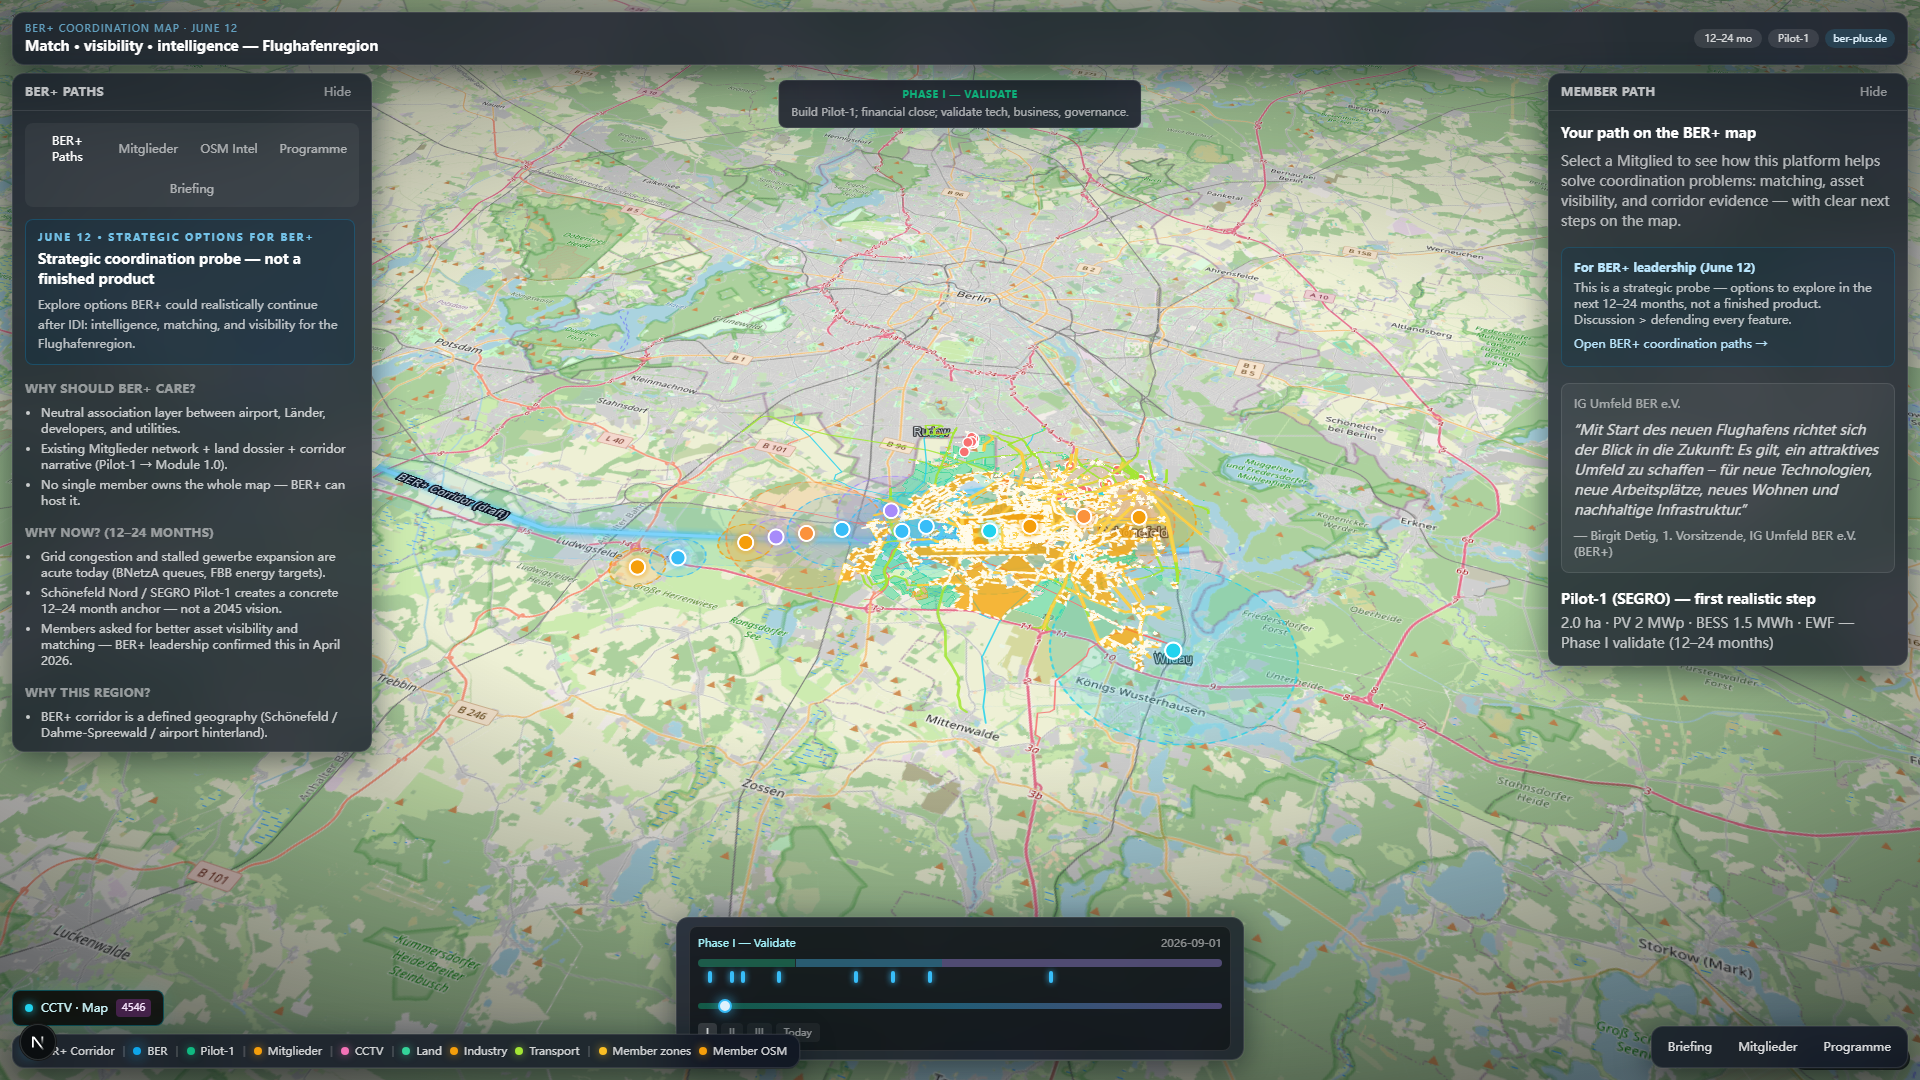
\includegraphics[width=\linewidth,height=0.72\textheight,keepaspectratio]{fig01-war-room-overview.png}
    \column{0.36\textwidth}
    \small
    \textbf{Ecosystem coordination}
    \begin{itemize}
      \item Corridor ribbon \& Pilot-1 timeline
      \item Mitglieder and influence zones
      \item OSM land, industry, power, transport
      \item Intelligence feed --- not a war room
    \end{itemize}
    \vspace{0.5em}
    \demourl
  \end{columns}
\end{frame}

% --- Demo: company ---
\begin{frame}{Demo --- company seeking a location}
  \begin{columns}[T]
    \column{0.64\textwidth}
    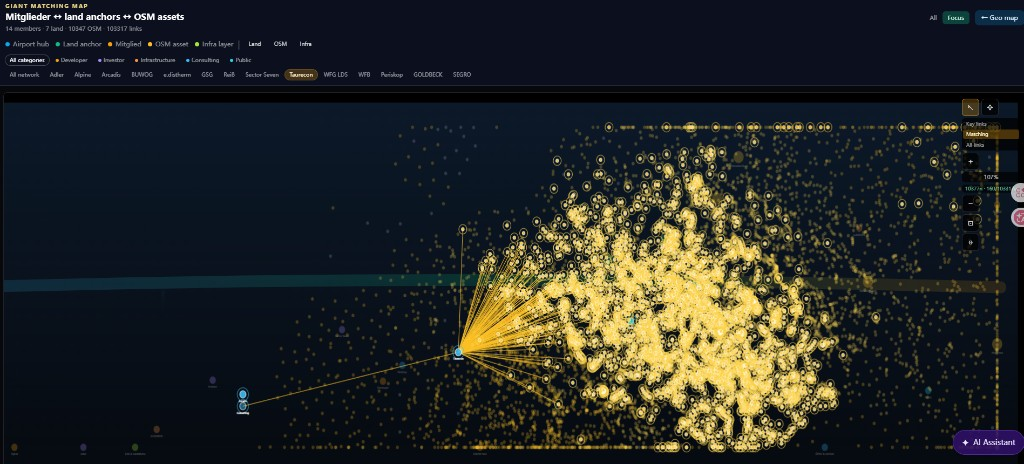
\includegraphics[width=\linewidth,height=0.72\textheight,keepaspectratio]{fig07-giant-matching-map.png}
    \column{0.34\textwidth}
    \small
    \textbf{Story on the map}
    \begin{itemize}
      \item Filter corridor layers
      \item Member focus --- scored links to land \& OSM
      \item Match review --- preview, Pass / Save
      \item \textit{Less talk --- show the prototype.}
    \end{itemize}
  \end{columns}
\end{frame}

% --- Demo: investor ---
\begin{frame}{Demo --- investor seeking opportunities}
  \begin{columns}[T]
    \column{0.48\textwidth}
    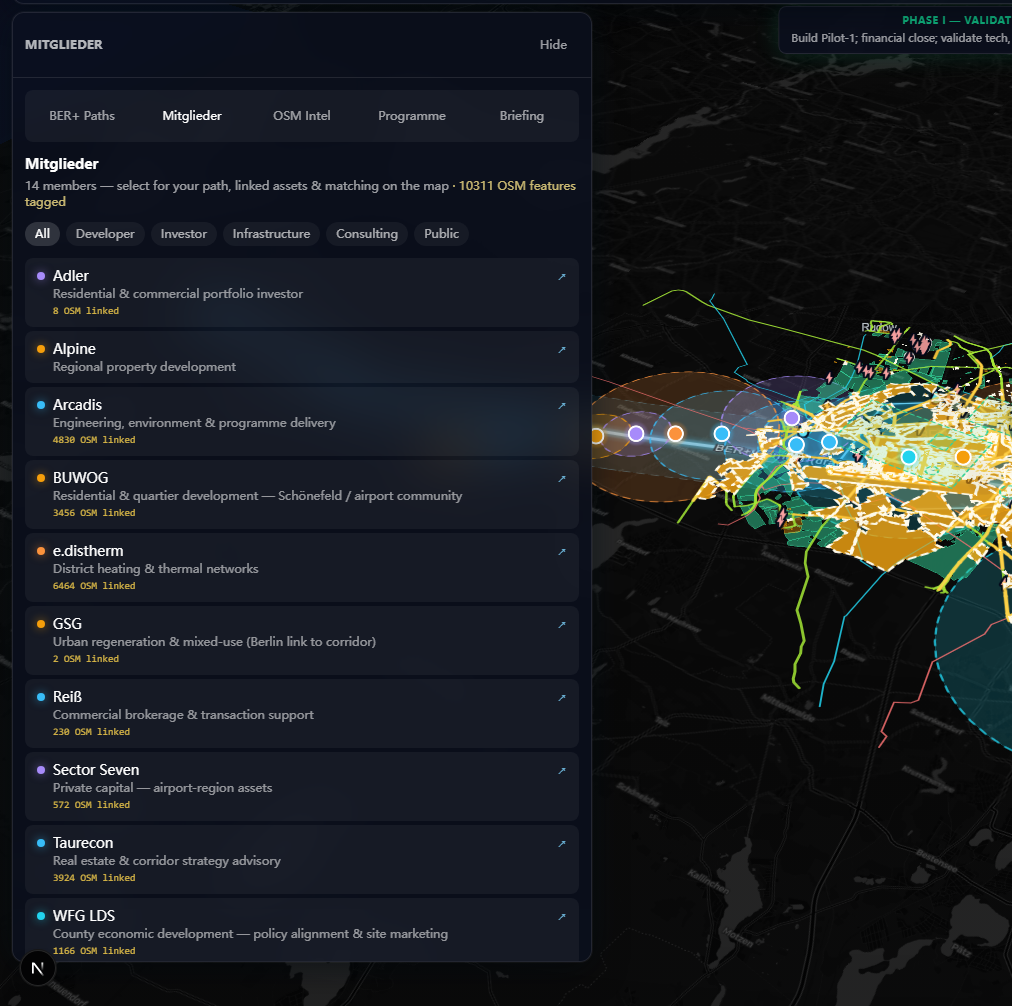
\includegraphics[width=\linewidth,height=0.7\textheight,keepaspectratio]{fig03-mitglieder-matching.png}
    \column{0.50\textwidth}
    \small
    \textbf{14 Mitglieder} --- developer, investor, infrastructure, consulting, public
    \begin{itemize}
      \item See link density per Mitglied
      \item Compare paths: BUWOG, SEGRO, WFG
      \item Qualified intros --- not cold outreach
    \end{itemize}
  \end{columns}
\end{frame}

% --- Demo: municipality / partners ---
\begin{frame}{Demo --- municipality \& partners}
  \begin{columns}[T]
    \column{0.62\textwidth}
    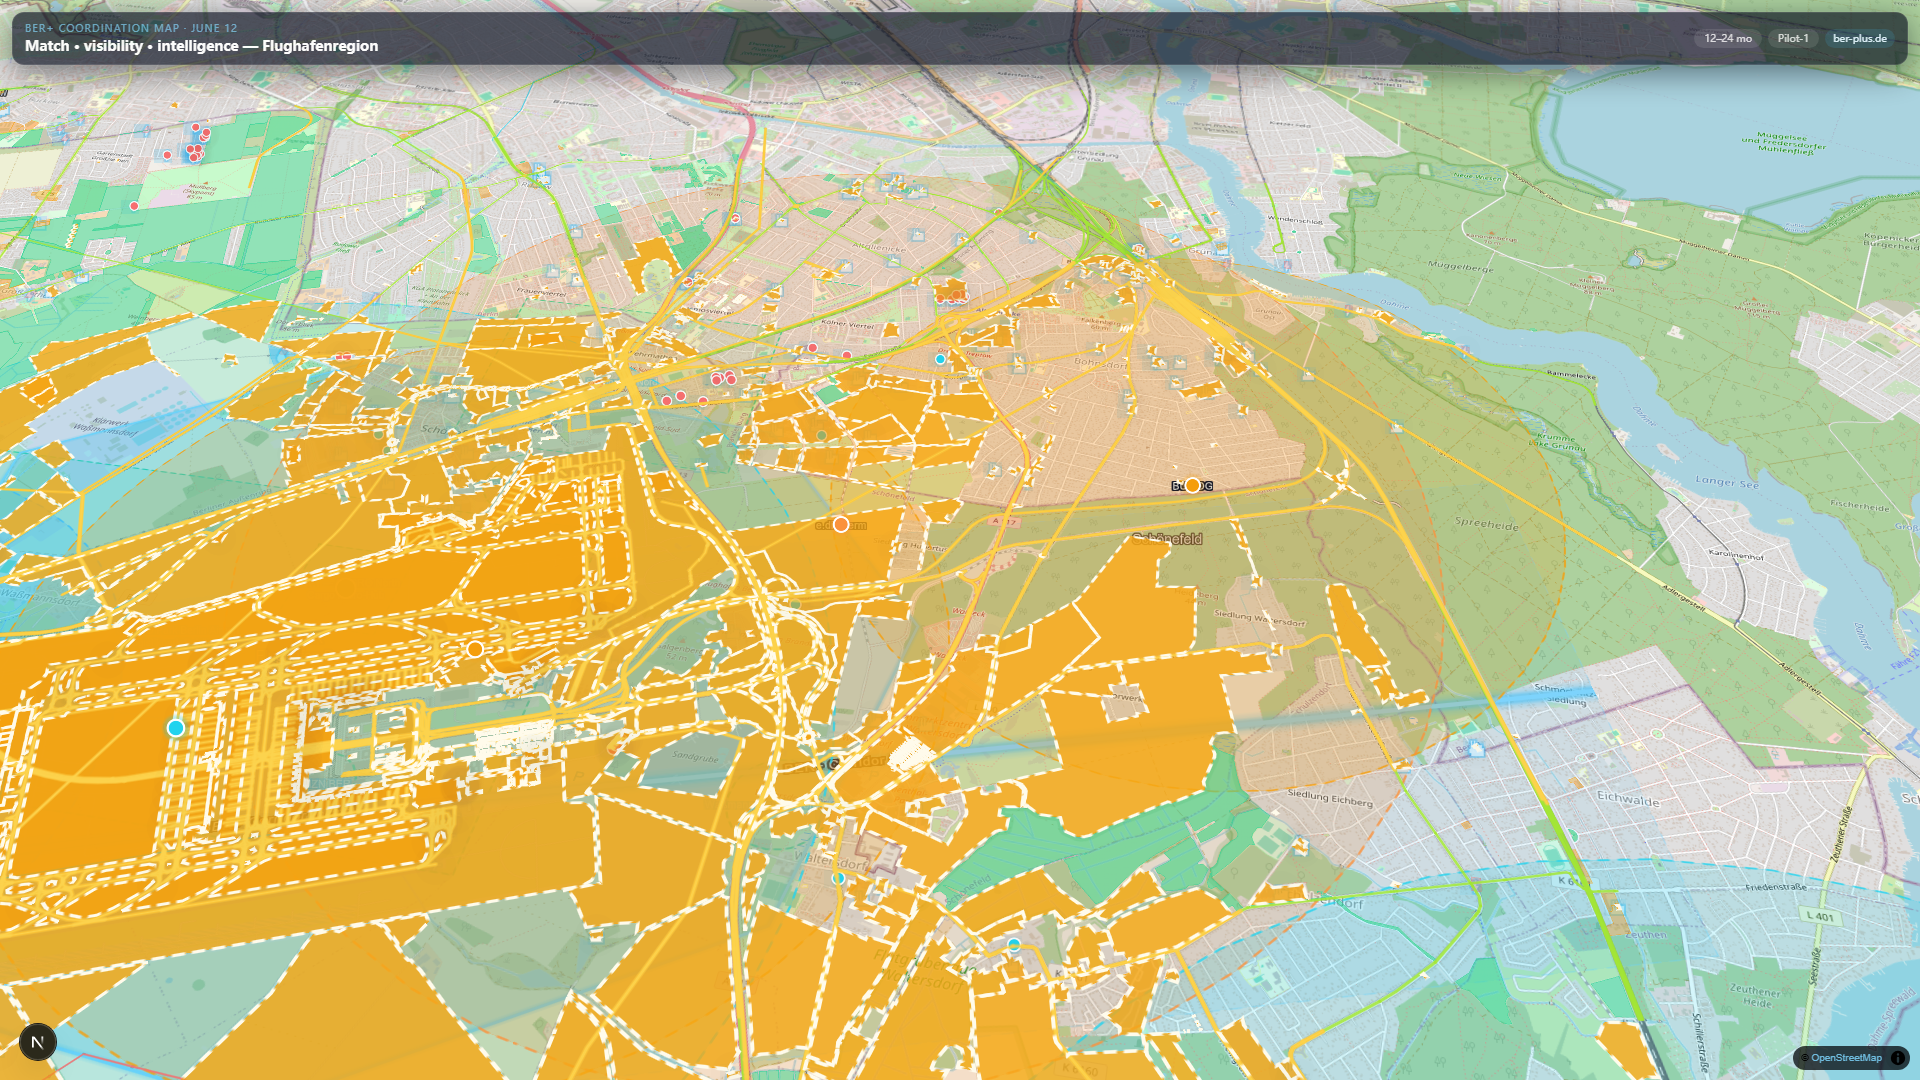
\includegraphics[width=\linewidth,height=0.72\textheight,keepaspectratio]{fig04-osm-intel.png}
    \column{0.36\textwidth}
    \small
    \textbf{OSM Intel}
    \begin{itemize}
      \item Land parcels \& suitability signals
      \item Industry, power, transport corridors
      \item Indicative layers --- planning stays with authorities
    \end{itemize}
  \end{columns}
\end{frame}

% --- Match review ---
\begin{frame}{Match review --- decide on the map}
  \begin{columns}[T]
    \column{0.58\textwidth}
    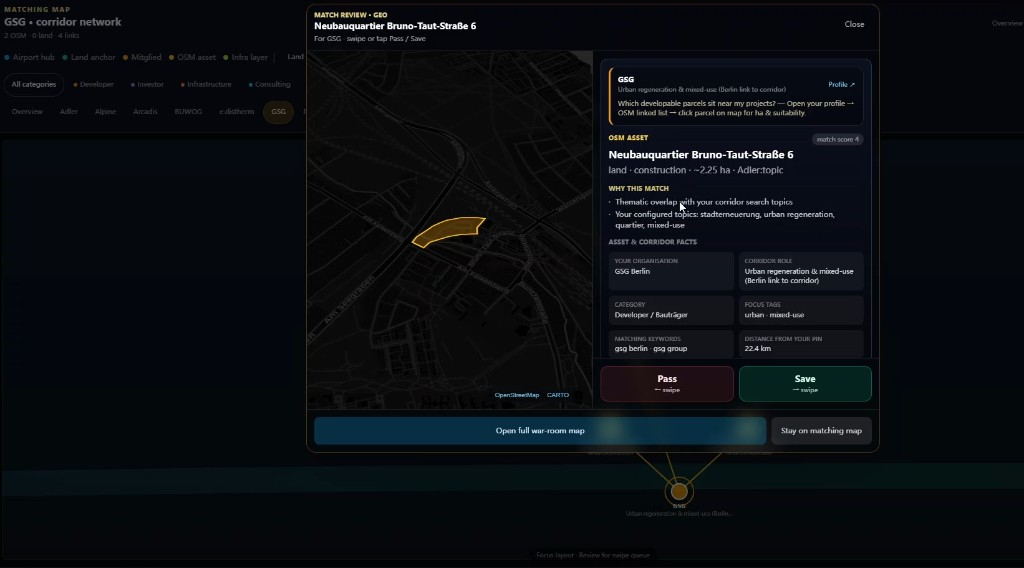
\includegraphics[width=\linewidth,height=0.72\textheight,keepaspectratio]{fig06-matching-review-popup.png}
    \column{0.40\textwidth}
    \small
    Tap any asset in member focus:
    \begin{itemize}
      \item Embedded site preview
      \item Match score and rationale
      \item Pass / Save --- stay in context
    \end{itemize}
  \end{columns}
\end{frame}

% --- Asset inventory ---
\begin{frame}{Next horizon --- what belongs to members?}
  \begin{itemize}
    \item Important follow-up: \textbf{member asset inventory}
    \item With Mitglieder, BER+ could build:
    \begin{itemize}
      \item Land inventory \quad infrastructure inventory
      \item Development opportunity inventory
    \end{itemize}
    \item Today's map is \textbf{step one} --- visibility and matching on open \& curated layers
    \item Pilot-1 (PV + BESS + EWF) anchors the programme timeline on the same surface
  \end{itemize}
\end{frame}

% --- BER+ pilot ---
\begin{frame}{What BER+ must do --- pilot phase}
  \begin{itemize}
    \item \textbf{Collect} --- member profiles, priorities, asset claims
    \item \textbf{Validate} --- locations and links with members (Arcadis, WFG, etc.)
    \item \textbf{Define} --- ownership of data refresh and matching rules
    \item \textbf{Maintain} --- quarterly OSM refresh, review queue
    \item \textbf{Host} --- neutral \berhub{} for board and member sessions
  \end{itemize}
  \vspace{0.3em}
  \small The platform is not magic --- BER+ makes it real.
\end{frame}

% --- BER+ future ---
\begin{frame}{Future phase --- how the platform evolves}
  \begin{itemize}
    \item Verified \textbf{member asset registry} linked to the map
    \item Matching at scale --- more Mitglieder, more rules, more exports
    \item Embedded in BER+ briefings, investor days, municipality sessions
    \item Intelligence packs and advocacy evidence from live map exports
  \end{itemize}
  \vspace{0.4em}
  \textbf{Goal:} ``We could start building this tomorrow.''
\end{frame}

% --- Discussion ---
\begin{frame}{Questions for the room}
  \begin{enumerate}
    \item Does the \textbf{problem framing} match your experience in the region?
    \item Which 3--5 Mitglieder pilot verified links first?
    \item Who owns the \textbf{asset inventory} conversation with members?
    \item First joint step after Pilot-1 --- hosting MOU, data refresh, matching group?
  \end{enumerate}
\end{frame}

% --- Close ---
\begin{frame}{Summary}
  \begin{itemize}
    \item \textbf{Problem first} --- fragmented visibility; \textbf{response} --- Coordination Map
    \item \textbf{Live today:} \demourl
    \item \textbf{Next:} pilot members, asset inventory dialogue, host the Hub
  \end{itemize}
\end{frame}

\begin{frame}[plain]
  \centering
  \Large Thank you\\[1.2em]
  \normalsize\demourl\\[0.6em]
  \small Live demo · questions
\end{frame}

\end{document}
